\subsection{A transition calibrated to falling AI-service prices}
\label{subsec:rewrite-price-calibration}

Table~\ref{tab:rewrite-price-parameters} distinguishes the empirical price
target from the assumed weights and initial efficiency.
\begin{rewriteParameterTable}{Price-calibrated transition: parameters and initial stocks}{tab:rewrite-price-parameters}
$\omega_X$ & 0.20 & AI production weight & Arbitrary post-change weight, not fitted to the industry's size; zero before date zero.\\
$\omega_L$ & 0.80 & Effective-labor weight & $1-\omega_X$; one before date zero.\\
$\chi$ & 51.760525 & Research productivity & Fitted at $\sigma=1$ to $p_X(2.25)/p_X(0)=0.20$; rounded OECD price decline, subject to the qualifications below \citep{oecdaimarkets2026}.\\
$\sigma$ & 0.90; 1; 1.10; 1.50 & AI--labor substitution & Arbitrary scenarios; only the unit-elastic price decline is fitted.\\
$\overline B$ & 170.1240 & AI-efficiency upper bound & $1.10\mathcal B(1.50)$; arbitrary margin above the analytical threshold.\\
\midrule
$A_0,N_0$ & 1; 1 & Initial technology and population & Unit normalizations.\\
$K_0$ & 5.941573 & Initial capital & Calculated no-AI Ramsey steady state, Equation~\eqref{eq:rewrite-ramsey-start-stocks}.\\
$B_0$ & 17.012402 & Initial AI efficiency & $0.10\overline B$; arbitrary assumption, not identified by the no-AI economy.\\
\end{rewriteParameterTable}

I now replace the illustrative transition-speed target with an observed
decline in AI-service prices. The OECD's quality-adjusted price index for
text-to-text models fell by nearly $80\%$ between January 2024 and April 2026
\citep{oecdaimarkets2026}. I use a rounded $80\%$ decline over 27 months as
the target for $p_X$. This is an approximate relative-price target: I hold
the price of the final good constant over the measurement window. The index
measures quality-adjusted cloud API prices, not the cost of completing a
fixed productive task. Competition, hardware improvements, and human research
also affect observed prices, so the exercise calibrates the model's timing
rather than separately identifying the productivity of RSI.

Before date zero, the economy is on the no-AI Ramsey steady state. I retain
its capital stock but set latent AI efficiency at $10\%$ of the upper bound:
\begin{equation}
 A_0=N_0=1,\qquad K_0=5.9416,\qquad
 B_0=0.10\overline B=17.0124.
 \label{eq:rewrite-price-calibration-stocks}
\end{equation}
The capital stock is calculated from the exact expression in
\eqref{eq:rewrite-ramsey-start-stocks}; the numbers above are rounded.
At date zero, the weights change from $(\omega_L,\omega_X)=(1,0)$ to
$(0.80,0.20)$, as in the preceding Ramsey-start experiment. I leave
$\eta=0.20$, $\overline B=170.1240$, and the macroeconomic parameters unchanged.
The initial efficiency ratio remains illustrative: it is not identified by
the pre-AI economy. Consumption and the shadow value are selected anew by
the BVP, not inherited from the Ramsey allocation.

I calibrate $\chi$ at $\sigma=1$, where the monopoly condition
\eqref{eq:rewrite-monopoly-foc} and the inverse-demand elasticity
\eqref{eq:rewrite-inverse-demand-elasticity} imply
\begin{equation}
 p_X=\frac{1}{(1-\alpha)\omega_X B},\qquad
 \frac{p_X(2.25)}{p_X(0)}=0.20.
 \label{eq:rewrite-price-calibration-target}
\end{equation}
Solving the equilibrium for each trial value gives $\chi\simeq51.76$,
compared with $1.4378$ in the main exercise. The price target implies
$B(2.25)=0.50\overline B$ in the unit-elastic case. I then hold this same
$\chi$ fixed across the four elasticities. The other three price declines
are predictions conditional on that calibration, not separately fitted
targets: over the same window, prices fall by $68.3\%$, $83.4\%$, and
$89.0\%$ for $\sigma=0.90,1.10,$ and $1.50$, respectively.

Figures~\ref{fig:rewrite-price-accumulation}--\ref{fig:rewrite-price-distribution}
use the same variables and normalizations as the preceding comparisons.
Each figure shows both the
first ten years and years 10--500, with separate vertical ranges
for the two windows. All four paths pass the equilibrium-admission tests,
including additional dense checks during the initial adjustment; the fitted
price ratio is unchanged to the reported precision after horizon refinement.

\begin{figure}[H]
 \centering
 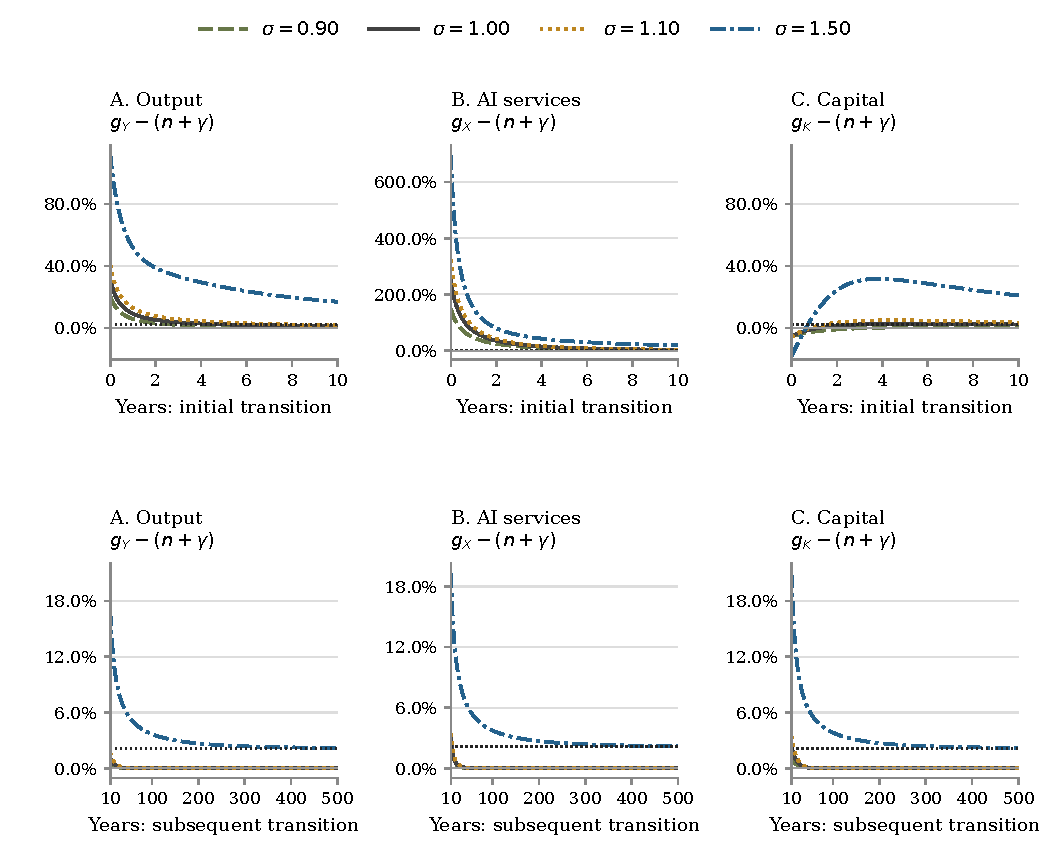
\includegraphics[width=\textwidth]{figures_rewrite/equilibrium_price_calibrated_accumulation_growth_windows.pdf}
 \caption{Price-calibrated transition: growth of output, AI production
 services, and capital per unit of effective labor. The upper row shows the
 first ten years; the lower row shows years 10--500. All growth
 rates are instantaneous annual rates, not realized one-year percentage
 changes. Panels A and C share a vertical scale within each row; Panel B
 has a separate range. Dotted horizontal lines mark the analytical limits
 for $\sigma=1.50$.}
 \label{fig:rewrite-price-accumulation}
\end{figure}

The faster improvement produces a sharp initial expansion, not a long period
of nearly unchanged growth. Initial output-per-person growth ranges from
$21.6\%$ at $\sigma=0.90$ to $113.2\%$ at $\sigma=1.50$; initial real-wage
growth ranges from $25.3\%$ to $54.4\%$. These are instantaneous annualized
rates. At $\sigma=1.50$, labor's share falls from $50.0\%$ at date zero to
$27.6\%$ after 27 months and $15.2\%$ after ten years. It completes half of
its decline toward zero in about three years, but reaching $90\%$ of the
decline still takes about 52 years. Rapid technological improvement does not
eliminate the subsequent capital-accumulation transition.

\begin{figure}[H]
 \centering
 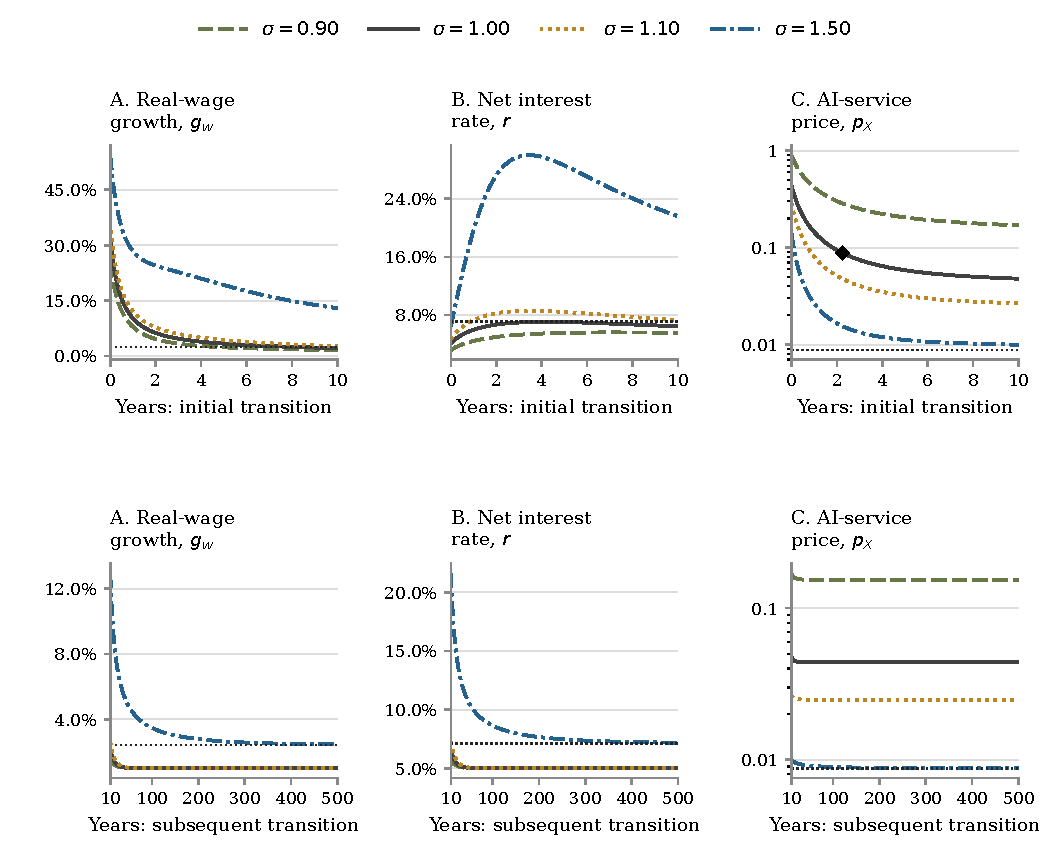
\includegraphics[width=\textwidth]{figures_rewrite/equilibrium_price_calibrated_growth_returns_windows.pdf}
 \caption{Price-calibrated transition: real-wage growth, the net interest
 rate, and the AI-service price. The upper row shows the first ten years;
 the lower row shows years 10--500. Rates use linear percentage scales and
 $p_X$ uses a logarithmic scale. The black diamond in the upper price panel
 marks the rounded OECD target, scaled to the model's initial unit-elastic
 price; it is not an observed absolute price in model units. Dotted lines
 mark the analytical limits for $\sigma=1.50$.}
 \label{fig:rewrite-price-returns}
\end{figure}

The financing response differs across regimes. At $\sigma=1$, research
initially uses $1.1\%$ of output: high research productivity permits rapid
efficiency gains without large research expenditure. At $\sigma=1.50$,
research instead absorbs $13.7\%$ of output and net profit is initially
$-3.9\%$ of output, or $-22.8\%$ of AI revenue. The household finances this
temporary loss against future monopoly profits. Capital per unit of
effective labor initially contracts, before the expansion in output finances
faster accumulation. The long-run regimes remain unchanged. By year 500,
the three labor-bottleneck economies have returned to approximately $1\%$
output-per-person and wage growth and a $5\%$ net interest rate. At
$\sigma=1.50$, the corresponding rates are $3.19\%$, $2.46\%$, and $7.18\%$,
approaching their analytical limits.

\begin{figure}[H]
 \centering
 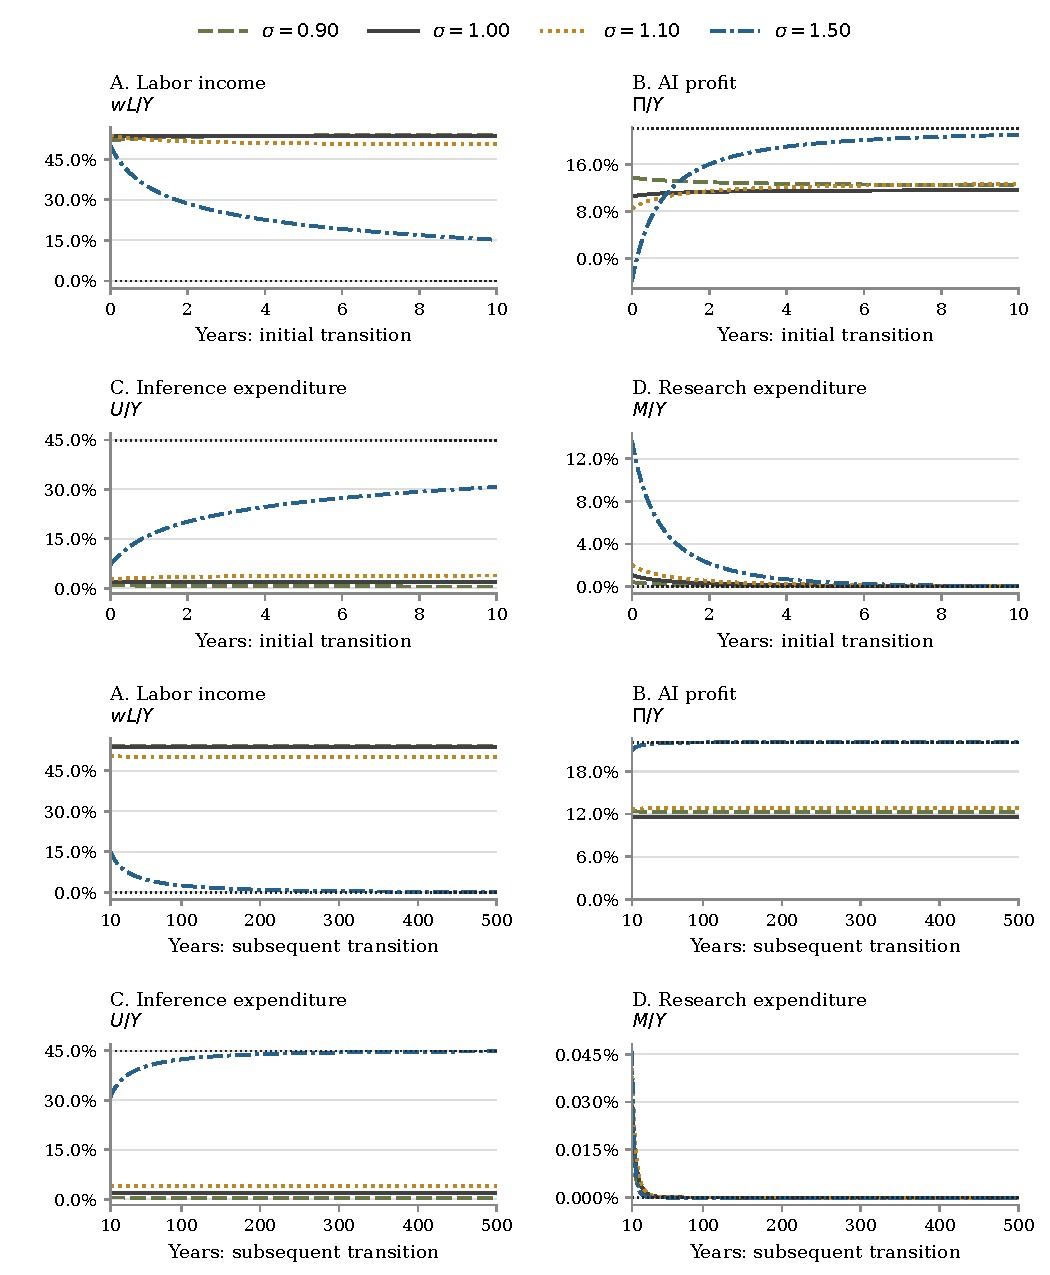
\includegraphics[width=\textwidth,height=0.83\textheight,keepaspectratio]{figures_rewrite/equilibrium_price_calibrated_ai_distribution_windows.pdf}
 \caption{Price-calibrated transition: labor income, AI net profit,
 inference expenditure, and research expenditure as shares of output.
 The first two rows show the first ten years; the last two show years 10--500.
 The four shares sum to $1-\alpha$; gross capital income remains $\alpha$.
 Negative AI profit denotes financing by the household owner. Vertical
 ranges differ between the two windows. Dotted lines mark the analytical
 limits for $\sigma=1.50$.}
 \label{fig:rewrite-price-distribution}
\end{figure}

\begin{samepage}
This exercise matches the price decline, not the current scale of the AI
industry or observed aggregate growth. Under the retained stocks and CES
weights, AI revenue already represents between $13.2\%$ and $17.0\%$ of
output at date zero. Combining that initial scale with rapid efficiency
improvement generates large immediate macroeconomic effects. The results
therefore describe a conditional equilibrium experiment, not a forecast
dated to January 2024. Matching the current industry's size as well as its
price decline would require a separate calibration of the initial technology
and production weights.

\end{samepage}
